\section{Methods}
\label{sec:methods}

Web Image Processing Pipeline (WIPP) is a scientific workflow engine,
illustrated as shown in figure 1. This tool enables all kinds of image
visualization and analysis. The workflow concept enables a sequence of plugins,
a piece of code put in the form of a container, allowing all kinds of analysis
or modification.

\begin{figure}[H]
  \centering
  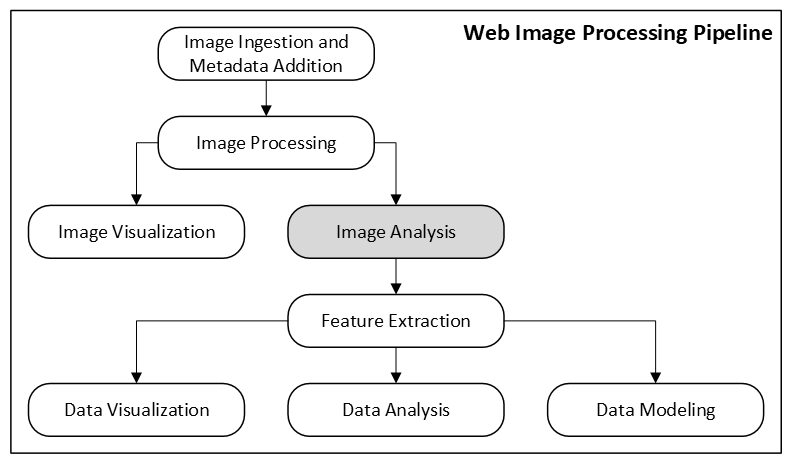
\includegraphics[width=0.8\linewidth]{png/1_wipp.png}
  \caption{Web Image Processing Pipeline}
  \label{fig:1wipp}
\end{figure}

Thanks to a plugin you can, for example, load an AI hosted in WIPP, specify an
image collection and perform the inference of this AI on the selected images.
The result will be a new collection of images modified by the AI, for example
with a label after inference of a classification model.

\subsection{Access public repositories via WIPP}

We have developed new inference plugins, see figure 2, to enable access to AI
models available on different public repositories.
\TODO ADD SAM2, ADD CELLPOSE here

\begin{figure}[H]
  \centering
  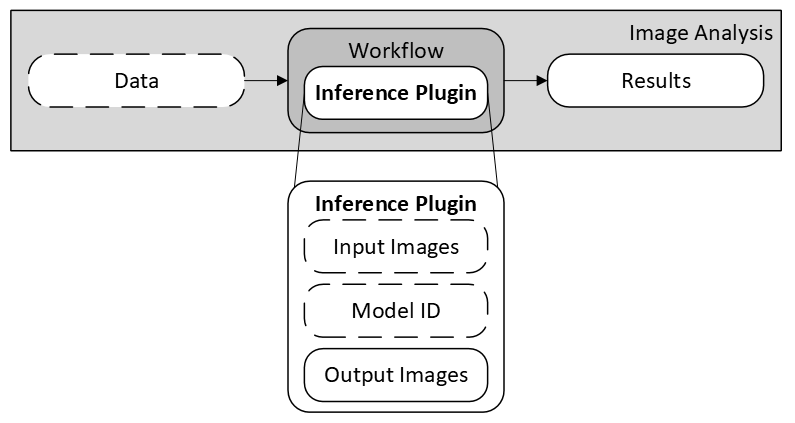
\includegraphics[width=0.8\linewidth]{png/2_inference_plugin.png}
  \caption{Inference Plugin}
  \label{fig:2inference}
\end{figure}

This was achieved by developing general-purpose code using the Application
Programming Interfaces (APIs) of the various platforms: Transformers for Hugging
Face and the BioImage.IO API. This enabled us to increase the number of
Artificial Intelligence (AI) models usable in WIPP thanks to containerized
software.

\subsection{Document AI models}

We have introduced AI model card entries that are necessary for matching tasks
with AI models. This information will also be needed as runtime parameters.
Figure 3, training an AI in WIPP automatically generates its documentation
(model card).

\begin{figure}[H]
  \centering
  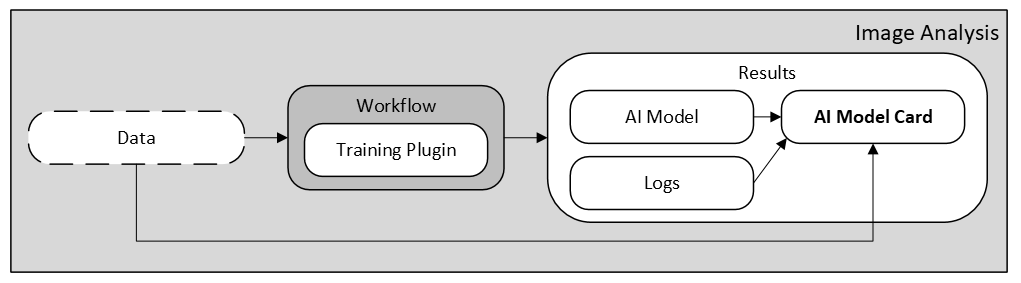
\includegraphics[width=0.8\linewidth]{png/3_ai_model_card.png}
  \caption{AI Model Card}
  \label{fig:3aimodelcard}
\end{figure}

This was achieved by developing code to retrieve information about the AI model
throughout the pipeline: name, creation date, data used for training, number of
iterations, training time, and more.

\subsection{Compute accuracy}

We have developed a new plugin, see figure 4, to compute the Dice-Sørensen
coefficient. It is a statistic used to gauge the similarity of two samples, in
our case images.

\begin{figure}[H]
  \centering
  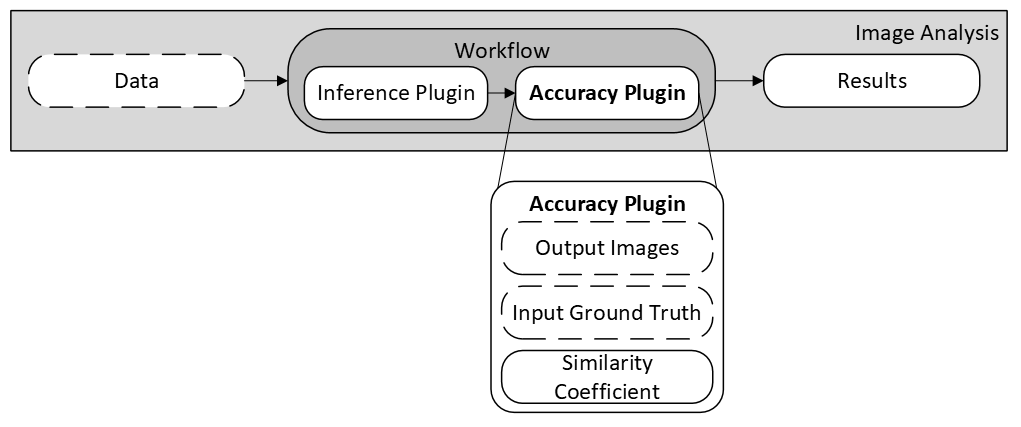
\includegraphics[width=0.8\linewidth]{png/4_accuracy.png}
  \caption{Accuracy Plugin}
  \label{fig:4accuracy}
\end{figure}

This was achieved by implementing the Sørensen's formula into a containerized
software (plugin). This makes it now possible to sequence model inference (a
model created within WIPP, as in workflow 1, or a model from a repository such
as Hugging Face, as in workflow 2) and evaluate the accuracy of the result
provided, by comparing it with ground truth data.
